\documentclass[10pt,a4paper]{article}

\usepackage{epsfig}
\usepackage{amsmath}
\usepackage{graphicx}
\usepackage{float}
\usepackage{subfig}
\usepackage{vmargin}
\usepackage{mathrsfs}
\usepackage{mathbbol}
\usepackage[parfill]{parskip}
\setmargrb{20mm}{20mm}{20mm}{20mm}

% Here enter any other preamble

\newcommand{\be}{\begin{equation}}
\newcommand{\ee}{\end{equation}}
\newcommand{\ba}{\begin{equation} \begin{aligned}}
\newcommand{\ea}{\end{aligned} \end{equation}}
\newcommand{\ddt}[1]{\frac{\mathrm{d}#1}{\mathrm{d}t}}
\newcommand{\indic}[1]{\mathbf{1}_{\{#1\}}}


%\newtheorem{mydef}[equation]{Definition}
\newtheorem{mydef}{Definition}

\title{\sc Household Isolation Model for COVID-19:\\
Context and Potential for HPC Acceleration}
\author{Thomas House}

\begin{document}

\maketitle

\section{Context and Importance}

Non-pharmaceutical interventions (NPIs) are a key tool that we have to fight
against COVID-19. While there are multiple models of most NPIs, to my knowledge
there is only one that explicitly includes isolation at the household level,
which is the influential study from Imperial College \cite{ferguson:2020}.  The
modelling methodology for this study is individual-based simulation, which
makes it slow and hard to run sensitivity analysis. The SPI-MO committee that
coordinates modelling work in the UK regards it as important to have multiple
models that investigate each question. Models are being developed at Lancaster
University and the London School of Hygiene and Tropical Medicine (LSHTM), but
this work is not completed. I have coded and disseminated a household model,
but the feedback on this is that additional sensitivity analysis would be
beneficial, and HPC would help with this.

The methodology involved is the use if self-consistent differential equations.
These were first written down (as were many firsts in household modelling) by
Frank Ball \cite{Ball:1999}. More recent developments, including numerical
methods for these equations, include
\cite{House:2008,Black:2017,Kinyanjui:2018}. The important features of this
approach is that it allows for the small, finite size of each household in
which random effects are important and each pair can only participate in
one infection event.

In the language of compartmental epidemic models, the dynamics are SEPIR
(susceptible, latent, mildly symptomatic prodrome, symptomatic infectious,
removed).

In general, within-household transmission needs to be scaled with household
size and the Cauchemez model where transmission $\propto$ size$^{-\eta}$  is
assumed.

The distribution of household sizes is realistic for the UK.

At present, an epidemic with no intervention is considered, then with three
weeks of global / non-household-based interventions of varied efficacy brought
in three weeks into the epidemic, as well as combination of different kinds of
isolation:

\begin{enumerate}
\item Individual isolation, where a proportion of individuals stay at home
when symptomatic.
\item Weak household isolation, where a proportion of households isolate when
there is at least one symptomatic individual in the household.
\item Strong household isolation, where a proportion of households isolates
from the first appearance of symptoms until 14 days after the end of all illness
in the household.
\end{enumerate}

The main model limitations that cannot be easily overcome in this framework are
determinism outside the household, lack of other spatial / risk structure
besides households, compartmental structure.

Another limitation where HPC methods could be very helpful is in systematic
assessment of sensitivity of the results. There are two kinds of such
sensitivity -- the first is multi-core runs of different scenarios (lengths and
types of non-household interventions, lengths and types of household isolation
policies). The other is sensitivity to the underlying rate constants, which I
think could be done by looking for the gradient of the outputs with respect to
the parameters, perhaps with autograd, in the first instance.  There is also
the possibility for hardware acceleration of the solution of the basic model,
which heavily depends on linear algebra.

\section{Formal model description}

Let $Q_{n,s,e,p,i,\mathbf{f}}(t)$ be the proportion of households in the
population at time $t$ of size $n$, with $s$ susceptiples, $e$ exposed, $p$
prodromal, and $i$ symptomatic infectious individuals, and with vector of
`flags' $\mathbf{f}$ representing implementation of more complex interventions.
The number of recovered individuals will be $n-s-e-p-i$ so we do not need to
index this explicitly. We now consider how to model different intervention
scenarios.

\subsection{Baseline}

In the absence of household-based interventions, we have
\ba
\ddt{}Q_{n,s,e,p,i} & = - \left(s r_{s\rightarrow e}(t,\mathbf{Q}) + e
r_{e\rightarrow p} + p r_{p\rightarrow i} + i r_{i\rightarrow \emptyset} 
+ n^{-\eta}s p \tau_p  + n^{-\eta}s i  \tau_i \right) Q_{n,s,e,p,i}
\\ & \qquad
+ (s+1) r_{s\rightarrow e}(t,\mathbf{Q}) Q_{n,s+1,e-1,p,i}
+ (e+1) r_{e\rightarrow p} Q_{n,s,e+1,p-1,i}
\\ & \qquad
+ (p+1) r_{p\rightarrow i} Q_{n,s,e,p+1,i-1}
+ (i+1) r_{i\rightarrow \emptyset} Q_{n,s,e,p,i+1}
\\ & \qquad
+ n^{-\eta}(s+1) p \tau_p Q_{n,s+1,e-1,p,i}
+ n^{-\eta}(s+1) i \tau_i Q_{n,s+1,e-1,p,i}
\text{ ,}
\ea
where we take any $Q$ with logically impossible indices just to equal $0$,
and the transmission into households is given by
\be
r_{s\rightarrow e}(t,\mathbf{Q}) = \Lambda(t) +
\sum_{n=1}^{n_{\mathrm{max}}}
\sum_{s=0}^{n}
\sum_{e=0}^{(n-s)}
\sum_{p=0}^{(n-s-e)}
\sum_{i=0}^{(n-s-e-p)}
\left(p \beta_p(t) + i \beta_i(t) \right) Q_{n,s,e,p,i}
\text{ .}
\ee
Here $\Lambda$ represents infections imported from outside the population of
households, and the other terms represent between-household transmissions.  We
take a `global' intervention as part of the baseline, in particular, we can
model phenomena such a school closures that hold during a set of times
$\mathcal{T}$ as
\be
\beta_x(t) = \begin{cases} (1-\varepsilon) \beta_x(0) & \text{ if } t \in \mathcal{T}
\text{ ,} \\
\beta_x(0) & \text{ otherwise,} \end{cases}
\ee
for $x \in \{p, i\}$. We call $\varepsilon$ the \textbf{global reduction}. We will
generally drop this $t$-indexing below, but it is present in all scenarios.

\subsection{Individual isolation}

We are then in a position to consider interventions. For individual isolation
we assume that a fraction $\alpha_{\mathrm{I}}$ , which we call the
\textbf{compliance}, of symptomatic cases self-isolates and ceases transmission
outside the household, but 
\be
r_{s\rightarrow e}(t,\mathbf{Q}) = \Lambda(t) +
\sum_{n=1}^{n_{\mathrm{max}}}
\sum_{s=0}^{n}
\sum_{e=0}^{(n-s)}
\sum_{p=0}^{(n-s-e)}
\sum_{i=0}^{(n-s-e-p)}
\left(p \beta_p + (1-\alpha_{\mathrm{I}}) i \beta_i \right) Q_{n,s,e,p,i}
\text{ .}
\ee

\subsection{Weak household isolation}

This corresponds to a situation where a fraction $\alpha_{\mathrm{W}}$ of
households isolate when there is at least one symptomatic case in the
household. These households do not experience new infections, meaning
that the dynamics become
\ba
\ddt{}Q_{n,s,e,p,i} & = - \left(
\left(1-\alpha_{\mathrm{W}} \indic{i>0} \right)s r_{s\rightarrow e}(t,\mathbf{Q})
+ e r_{e\rightarrow p} + p r_{p\rightarrow i} + i r_{i\rightarrow \emptyset} 
+ n^{-\eta}s p \tau_p  + n^{-\eta}s i  \tau_i \right) Q_{n,s,e,p,i}
\\ & \qquad
+ \left(1-\alpha_{\mathrm{W}} \indic{i>0} \right)
(s+1) r_{s\rightarrow e}(t,\mathbf{Q}) Q_{n,s+1,e-1,p,i}
+ (e+1) r_{e\rightarrow p} Q_{n,s,e+1,p-1,i}
\\ & \qquad
+ (p+1) r_{p\rightarrow i} Q_{n,s,e,p+1,i-1}
+ (i+1) r_{i\rightarrow \emptyset} Q_{n,s,e,p,i+1}
\\ & \qquad
+ n^{-\eta}(s+1) p \tau_p Q_{n,s+1,e-1,p,i}
+ n^{-\eta}(s+1) i \tau_i Q_{n,s+1,e-1,p,i}
\text{ ,}
\ea
and also do not transmit outside, meaning that the rate of between-household
transmission becomes
\be
r_{s\rightarrow e}(t,\mathbf{Q}) = \Lambda(t) +
\sum_{n=1}^{n_{\mathrm{max}}}
\sum_{s=0}^{n}
\sum_{e=0}^{(n-s)}
\sum_{p=0}^{(n-s-e)}
\sum_{i=0}^{(n-s-e-p)}
\left(1-\alpha_{\mathrm{W}} \indic{i>0} \right) \left(p \beta_p + i \beta_i \right)
 Q_{n,s,e,p,i}
\text{ .}
\ee

\subsection{Strong household isolation}

We now suppose that a fraction $\alpha_{\mathrm{S}}$ of households start to
isolate when there is at least one symptomatic case in the household, and stop
isolation 14 days after the absence of symptoms in the household. This is
modelled by having a flag $f=0$ if the household is not isolating and $f=1$ if
it is. The dynamics become
\ba
\ddt{}Q_{n,s,e,p,i,f} & = - \left(\indic{f=0}s r_{s\rightarrow e}(t,\mathbf{Q}) + e
r_{e\rightarrow p} + p r_{p\rightarrow i} + i r_{i\rightarrow \emptyset} 
+ n^{-\eta}s p \tau_p  + n^{-\eta}s i  \tau_i 
+ \indic{f=1} \sigma \right) Q_{n,s,e,p,i,f}
\\ & \qquad
+ \indic{f=0}(s+1) r_{s\rightarrow e}(t,\mathbf{Q}) Q_{n,s+1,e-1,p,i,f}
+ (e+1) r_{e\rightarrow p} Q_{n,s,e+1,p-1,i,f}
\\ & \qquad
+ (1-\indic{f=1 \& i=1 \& s+e+p=n-1} \alpha_{\mathrm{S}})
(p+1) r_{p\rightarrow i} Q_{n,s,e,p+1,i-1,f}
+ (i+1) r_{i\rightarrow \emptyset} Q_{n,s,e,p,i+1,f}
\\ & \qquad
+ n^{-\eta}(s+1) p \tau_p Q_{n,s+1,e-1,p,i,f}
+ n^{-\eta}(s+1) i \tau_i Q_{n,s+1,e-1,p,i,f}
\\ & \qquad
+ \indic{f=0} \sigma Q_{n,s,e,p,i,1}
+ \indic{f=1 \& i=1 \& s+e+p=n-1} \alpha_{\mathrm{S}}
(p+1)r_{p\rightarrow i} Q_{n,s,e,p+1,i-1,0}
\text{ ,}
\ea
with between-household term
\be
r_{s\rightarrow e}(t,\mathbf{Q}) = \Lambda(t) +
\sum_{n=1}^{n_{\mathrm{max}}}
\sum_{s=0}^{n}
\sum_{e=0}^{(n-s)}
\sum_{p=0}^{(n-s-e)}
\sum_{i=0}^{(n-s-e-p)}
\left(p \beta_p + i \beta_i \right) Q_{n,s,e,p,i,0}
\text{ .}
\ee

\bibliography{mybib}
\bibliographystyle{abbrv}


\clearpage

\section*{Figures}

\begin{figure}[H]
\begin{center}
  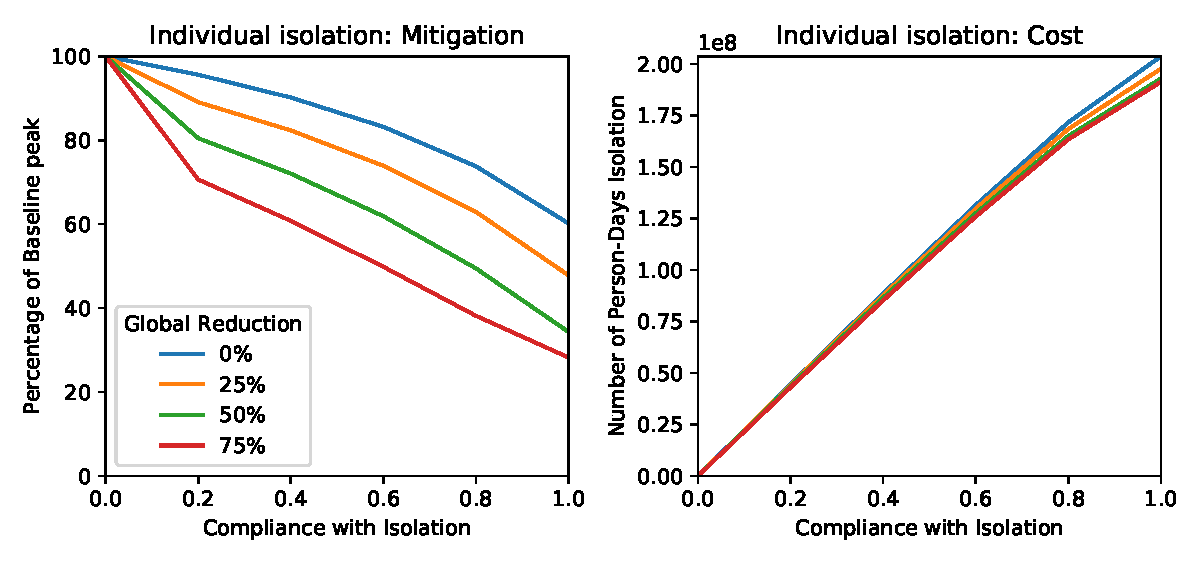
\includegraphics[width=0.8\textwidth]{figures/mit_costs.pdf}\\
  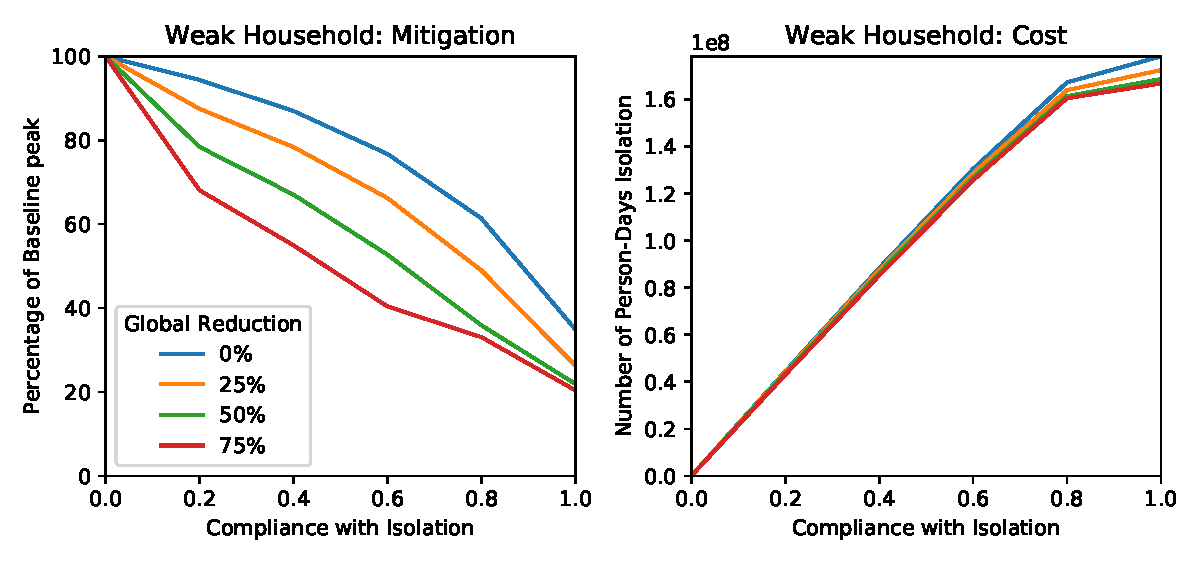
\includegraphics[width=0.8\textwidth]{figures/mit_costs_weak.pdf}\\
  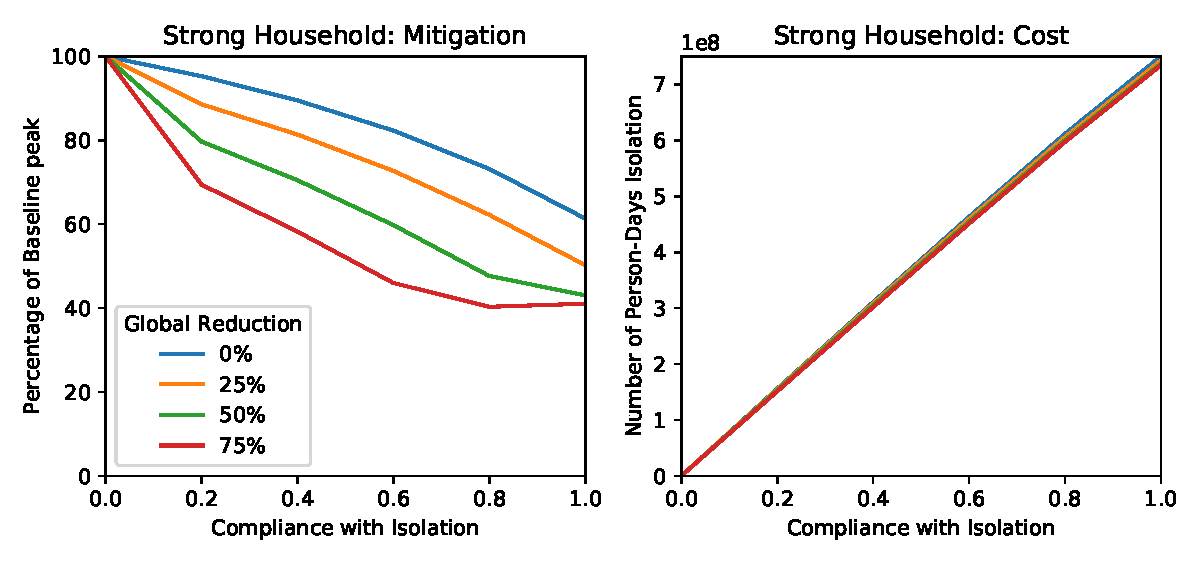
\includegraphics[width=0.8\textwidth]{figures/mit_costs_strong.pdf}
\end{center}
\caption{Results of different strategies on the peak height, and also
social cost of those interventions as person-days in isolation.}
\end{figure}

\clearpage

\section{Figures -- Vulnerable Individuals}

\begin{figure}[H]
\begin{center}
  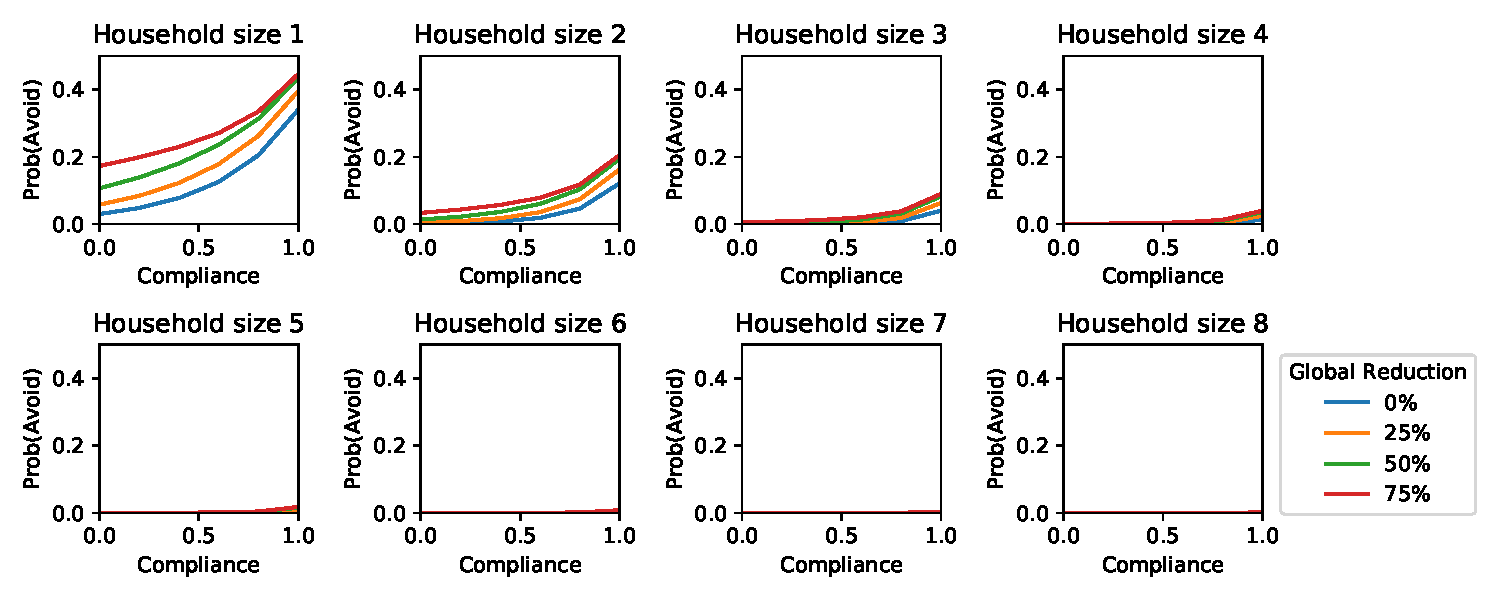
\includegraphics[width=0.8\textwidth]{figures/prob_avoid.pdf}
\end{center}
\caption{Probability of escape by household size for individual isolation.}
\end{figure}

\begin{figure}[H]
\begin{center}
  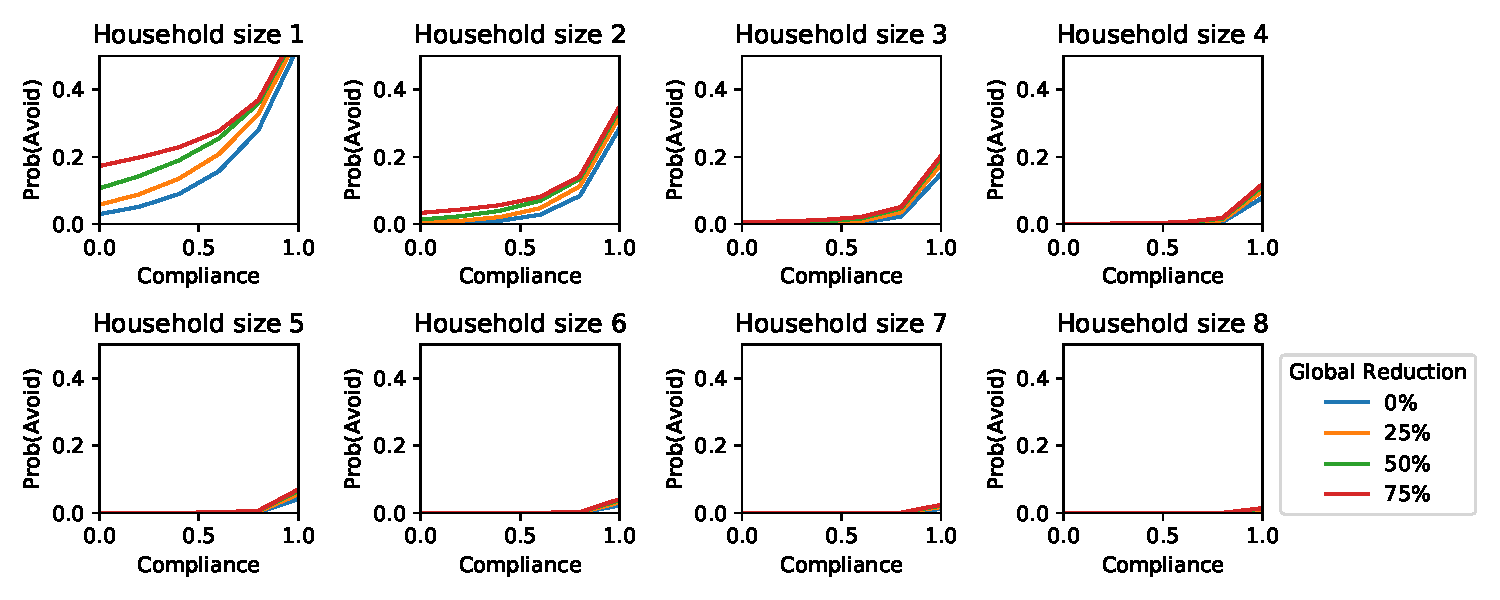
\includegraphics[width=0.8\textwidth]{figures/prob_avoid_weak.pdf}
\end{center}
\caption{Probability of escape by household size for weak household isolation.}
\end{figure}

\begin{figure}[H]
\begin{center}
  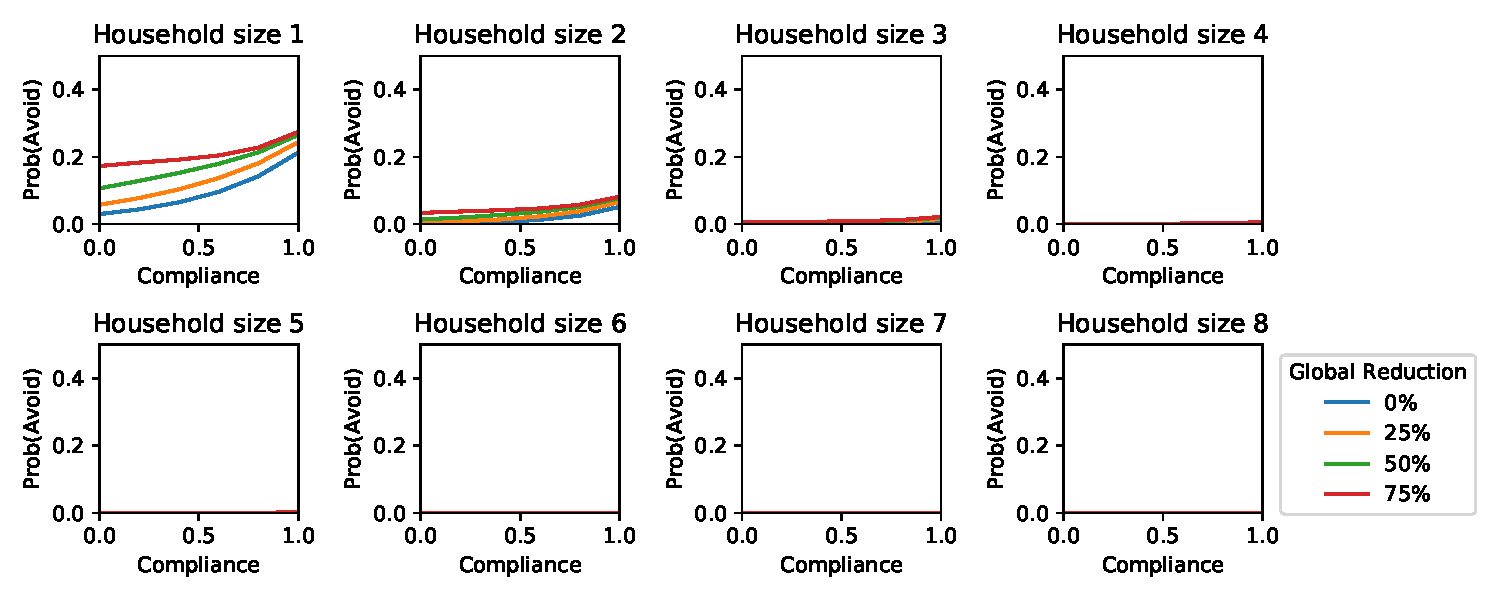
\includegraphics[width=0.8\textwidth]{figures/prob_avoid_strong.pdf}
\end{center}
\caption{Probability of escape by household size for strong household isolation.}
\end{figure}

\clearpage


\begin{figure}[H]
\begin{center}
  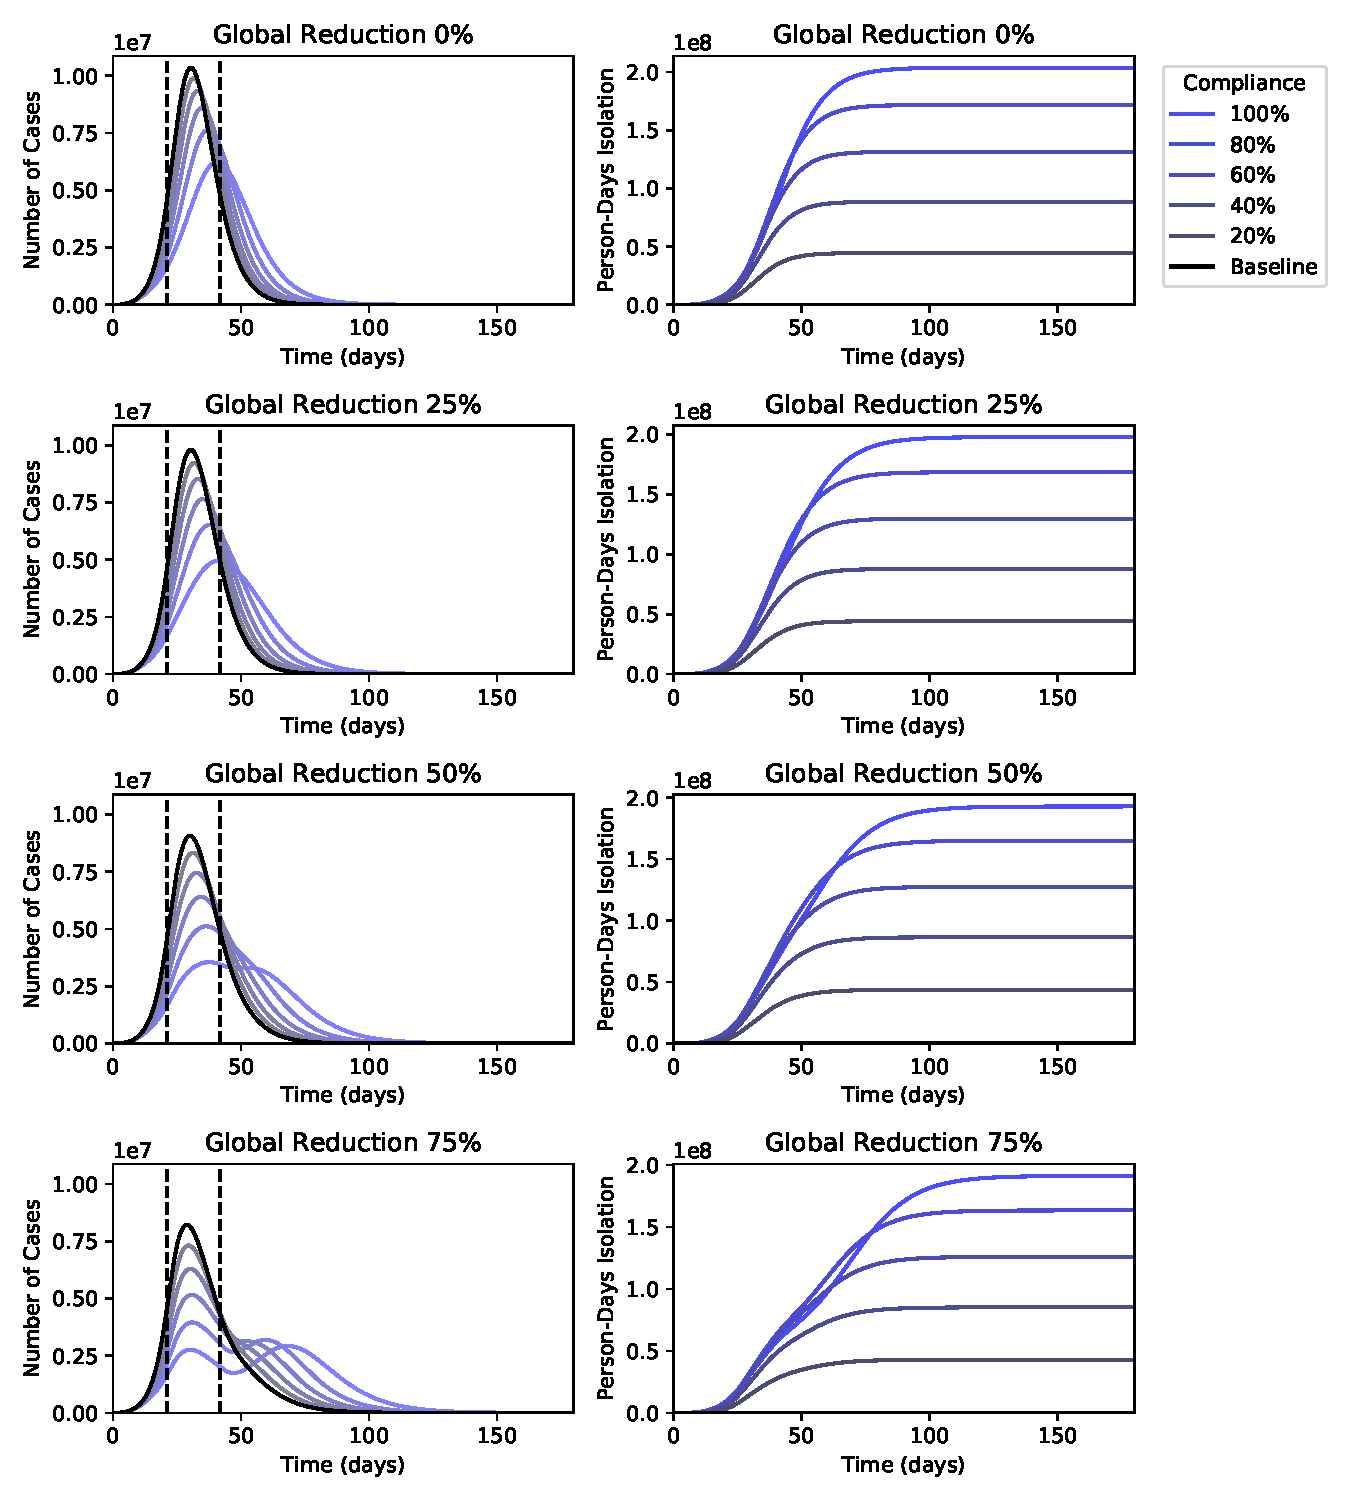
\includegraphics[width=0.99\textwidth]{figures/time_series.pdf}
\end{center}
\caption{Temporal behaviour for individual isolation.}
\end{figure}

\clearpage


\begin{figure}[H]
\begin{center}
  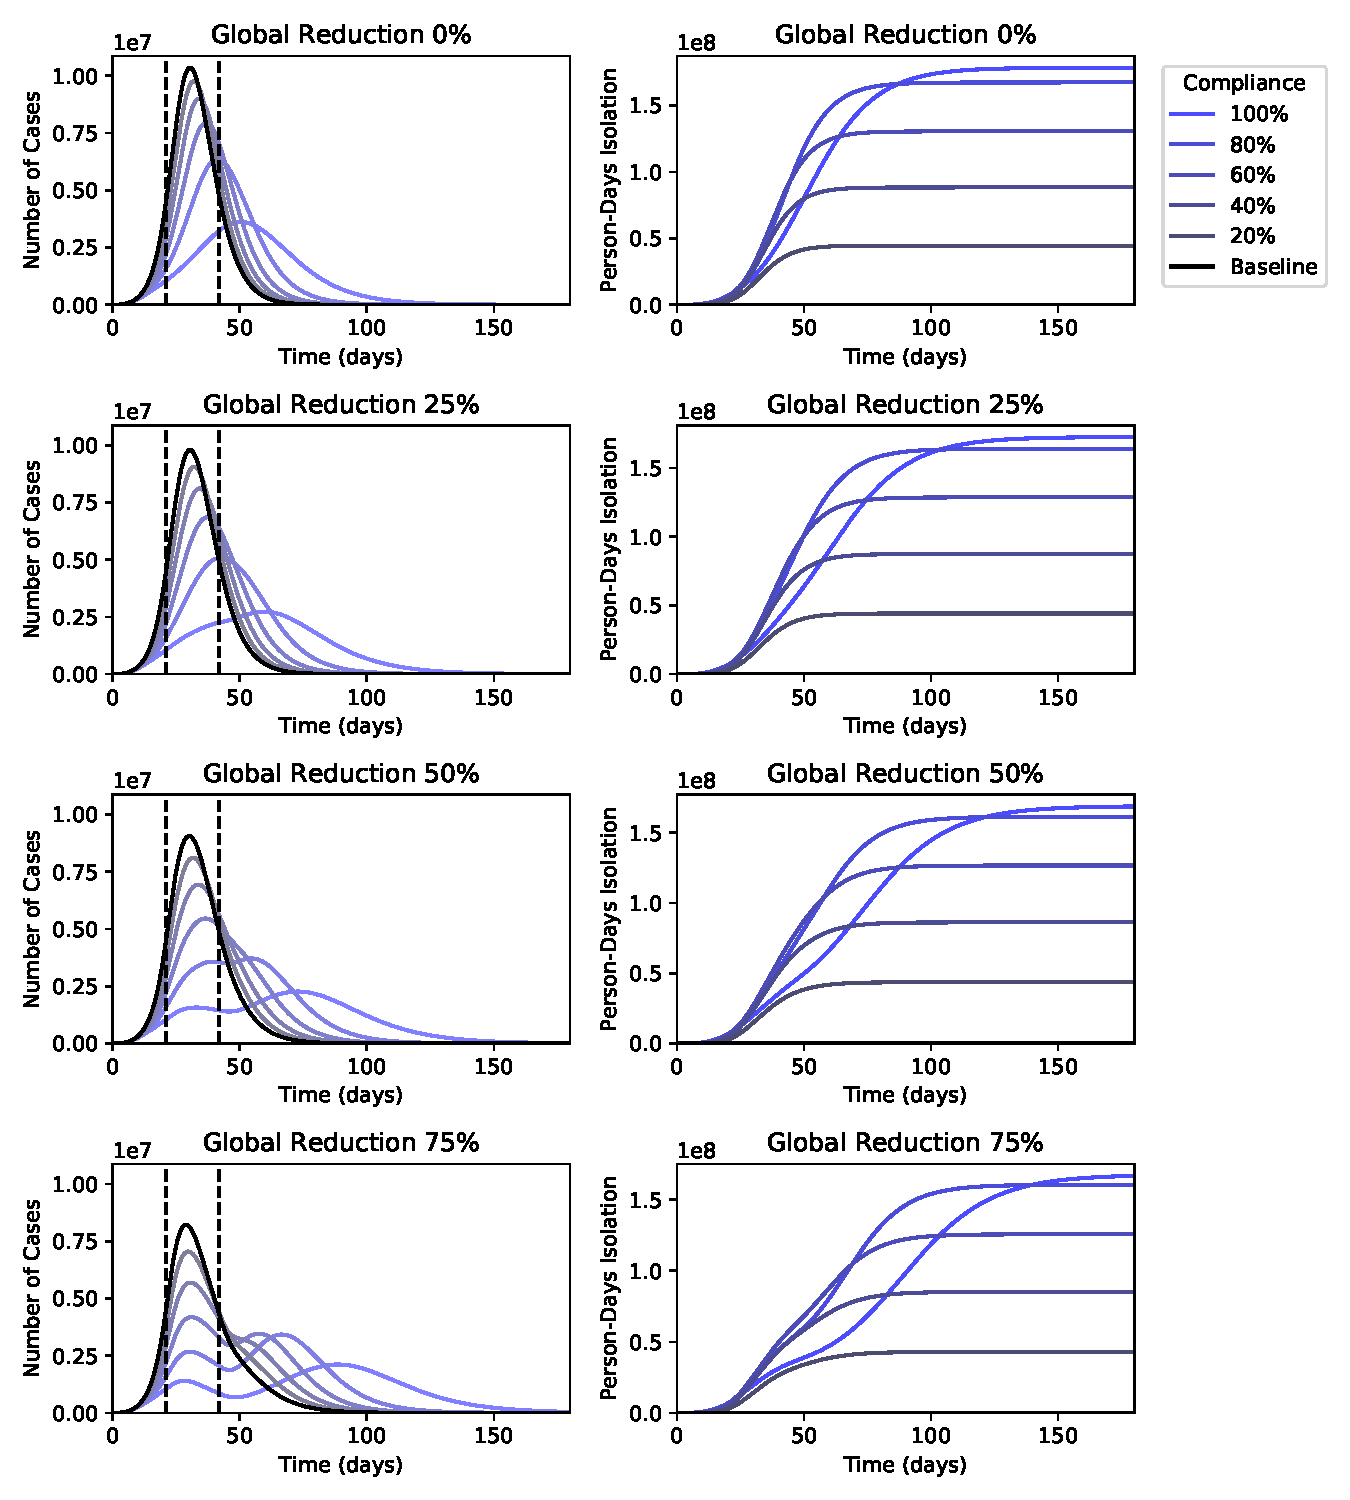
\includegraphics[width=0.99\textwidth]{figures/time_series_weak.pdf}
\end{center}
\caption{Temporal behaviour for weak household isolation.}
\end{figure}

\clearpage


\begin{figure}[H]
\begin{center}
  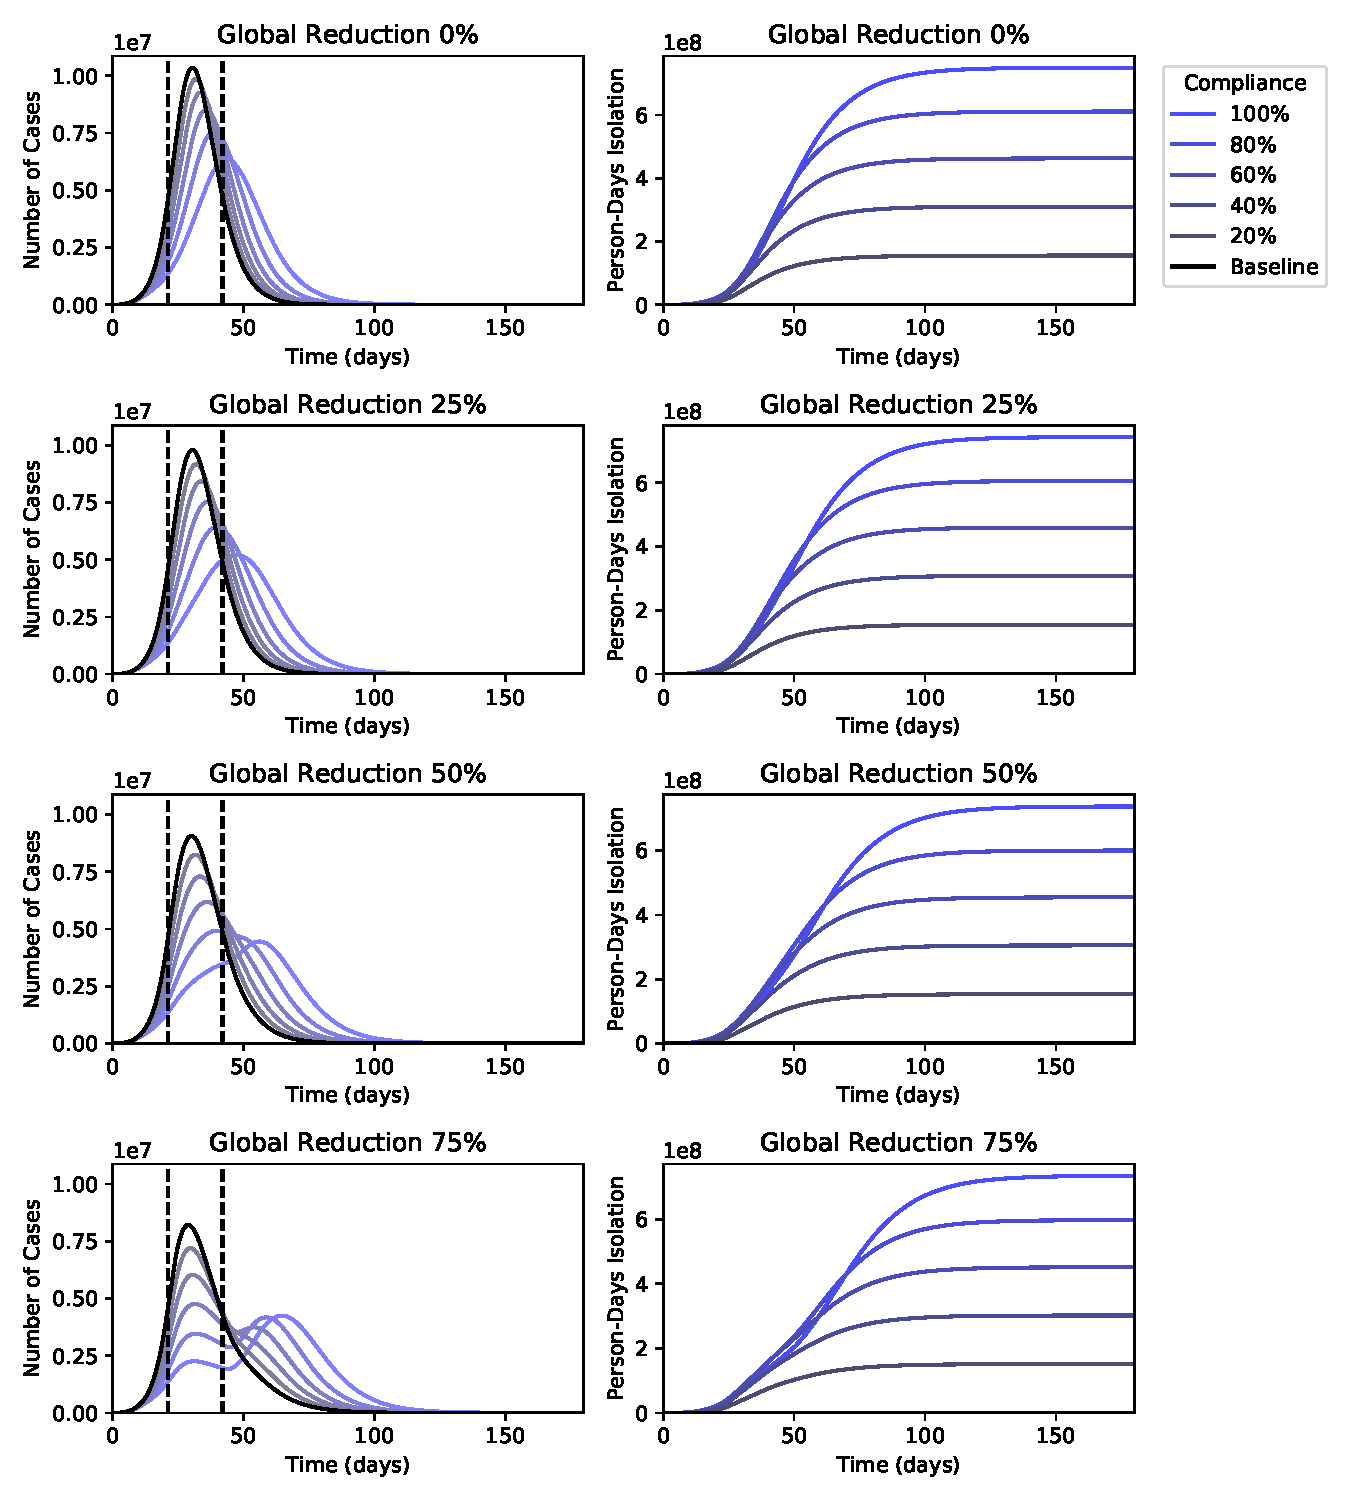
\includegraphics[width=0.99\textwidth]{figures/time_series_strong.pdf}
\end{center}
\caption{Temporal behaviour for strong household isolation.}
\end{figure}


\end{document}



